\documentclass{article}

% --- Packages ---
\usepackage[preprint]{neurips_2024}
\usepackage[utf8]{inputenc}
\usepackage[T1]{fontenc}
\usepackage{hyperref}
\usepackage{url}
\usepackage{booktabs}
\usepackage{amsmath}
\usepackage{graphicx}
\usepackage{subcaption}
\usepackage{multirow}
\usepackage{xcolor}
\usepackage{microtype}
\usepackage{natbib}

% ---------------------------------------------------------------------------
\title{Direct Imitation Learning for Autonomous Driving:\\
When the World-Model Latent Loses the Lane}

\author{
  Shilo Jeyarajasingam \\
  University of Waterloo $\cdot$ Independent Researcher \\
  \texttt{stjeyara@uwaterloo.ca}
}

\begin{document}
\maketitle

% ---------------------------------------------------------------------------
\begin{abstract}
World-model-based approaches to autonomous driving compress sensory
observations into a compact latent state before learning a policy.
We show that on the MetaDrive simulator \citep{li2022metadrive}, a
DreamerV3-style recurrent world model \citep{hafner2023dreamerv3}
loses the lane/heading signal in its latent representation, causing any
latent-conditioned policy to idle regardless of how much data or compute
is invested in it (route completion 2\%, vs.\ 22\% for a direct
obs$\to$action clone). Pivoting to direct behavioral cloning from a
259-dimensional state vector with a three-layer MLP reveals a different
ceiling: distribution shift. The policy commits to driving but goes
off-road 50\% of the time because it has only seen the expert driving
perfectly. We show that injecting triangular steering perturbations
(DART; \citealt{laskey2017dart}) during expert collection and relabeling
with the IDM oracle \citep{treiber2000idm} cuts off-road rate from 50\%
to 30\% and raises route completion from 24\% to 39\%. A per-scene
breakdown reveals that this aggregate masks near-expert performance on
three of four geometry types (straight 96\%, curve 87\%, intersection
84\%) while a single geometry --- roundabouts --- accounts for nearly all
remaining failures (route 42\%, off-road 60\%). Scene-targeted data
augmentation raises roundabout route completion to 64\% (+22 percentage
points) without regressing other scenes. Three iterations of DAgger with
IDM relabeling match but do not exceed the plain BC + augmentation
baseline, as growing dataset heterogeneity raises behavioral cloning loss
and causes regression by iteration 3. We conclude that for CPU-scale
imitation learning in simulation, targeted scene augmentation is a more
stable improvement lever than online DAgger. All code and trained
checkpoints are available at
\url{https://github.com/shilojeyaraj/driving-world-model}.
\end{abstract}

% ---------------------------------------------------------------------------
\section{Introduction}
\label{sec:intro}

Learning to drive from demonstrations is a canonical imitation learning
problem \citep{pomerleau1989alvinn}. Modern approaches follow one of two
paradigms: (1) learn a world model that predicts future latent states under
imagined actions, then optimise a policy against those imaginations
\citep{hafner2023dreamerv3,wu2023daydreamer}; or (2) clone a policy
directly from observations to actions using an expert oracle
\citep{codevilla2018conditional,chen2022learning}. The world-model paradigm
is theoretically attractive --- imagination-based planning can explore
policies without executing dangerous actions in the real environment ---
but relies critically on the latent representation preserving the
information the policy needs.

In this work we study what happens when the latent representation fails to
preserve that information. On the MetaDrive procedural driving simulator
\citep{li2022metadrive}, we train a DreamerV3-style RSSM
\citep{hafner2019rssm} on 8{,}000 steps of expert IDM demonstrations.
We then train a policy on the frozen world-model latent via behavioral
cloning. The result is an agent that idles: route completion 2\%,
behavioral cloning loss 2.06. Crucially, the observation space is
a 259-dimensional vector that already contains the full lane/heading
signal explicitly --- the world model is compressing it away rather
than enriching it. A three-layer MLP cloned \emph{directly} from
the 259-dim state to a 2-dim action (steering, throttle) achieves
bc\_loss 0.05 and route completion 22\%--24\% out of the box.

This reframing shifts the bottleneck from \emph{representation} to
\emph{distribution shift}: behavioral cloning fails not because the
policy lacks information, but because it has only seen the expert
driving cleanly along the lane center and therefore cannot recover
once it drifts. The rest of this paper characterises and addresses this
gap through three levers: recovery data injection (DART perturbation),
targeted scene augmentation, and online data aggregation (DAgger).

Our contributions are:
\begin{enumerate}
  \item An empirical demonstration that a DreamerV3-style world model on
    vector observations loses the lane signal in its latent, making
    latent-conditioned policies unable to drive regardless of training
    budget.
  \item A recovery data protocol using triangular steering perturbation
    (DART) and IDM relabeling that cuts off-road rate by 40\% relative
    ($50\%\to30\%$) and increases route completion from 24\% to 39\%.
  \item A per-scene diagnostic revealing that aggregate route metrics mask
    near-expert performance on most geometry types; a single geometry
    (roundabouts) dominates the residual gap.
  \item A scene-targeted augmentation strategy that raises roundabout
    route completion by 22 percentage points while preserving performance
    on all other scenes.
  \item An empirical comparison of DAgger vs.\ static augmentation at
    CPU-scale, showing that DAgger matches but does not exceed the
    augmented BC baseline and regresses by iteration 3 due to dataset
    heterogeneity.
\end{enumerate}

% ---------------------------------------------------------------------------
\section{Related Work}
\label{sec:related}

\paragraph{Imitation learning for autonomous driving.}
ALVINN \citep{pomerleau1989alvinn} introduced behavioral cloning for
driving from camera images. \citet{ross2011dagger} formalised Dataset
Aggregation (DAgger) to address distribution shift by iteratively querying
the expert at states visited by the current policy. ChauffeurNet
\citep{bansal2019chauffeurnet} augments demonstrations with synthesised
perturbations and auxiliary loss heads to improve recovery behaviour.
Our work applies these ideas in a low-compute, simulation-only setting
using the Intelligent Driver Model as the oracle.

\paragraph{World models for driving.}
DreamerV3 \citep{hafner2023dreamerv3} learns a recurrent world model (RSSM)
by jointly optimising a reconstruction decoder, a reward predictor, and a
discount predictor, then derives a policy by imagining rollouts in latent
space. DayDreamer \citep{wu2023daydreamer} applies this to real robot
learning. MILE \citep{hu2022mile} and UniAD \citep{hu2023uniad} learn
latent representations jointly with driving objectives. Our failure case
--- a world model that compresses away the precise signal the policy needs
--- is a known risk with RSSM-based representations when the observation
space is already low-dimensional and the model is under-trained.

\paragraph{Distribution shift in behavioral cloning.}
\citet{ross2010efficient} prove that BC error compounds quadratically with
horizon length. DAgger \citep{ross2011dagger} corrects this by
on-policy data collection; DART \citep{laskey2017dart} injects noise
to force the policy into off-distribution states during collection,
providing recovery labels without requiring online expert querying.
We combine both approaches and compare their effectiveness at modest
compute.

\paragraph{MetaDrive.}
MetaDrive \citep{li2022metadrive} is a lightweight, procedurally generated
driving simulator with a modular road block system supporting diverse
geometry types (straight, curve, intersection, roundabout). Its
Intelligent Driver Model (IDM; \citealt{treiber2000idm}) provides
a rule-based expert oracle that can be queried at arbitrary states,
making it ideal for DAgger and relabeling experiments.

% ---------------------------------------------------------------------------
\section{Methods}
\label{sec:methods}

\subsection{Environment and Observation Space}

All experiments use MetaDrive's \texttt{MetaDriveEnv} with 50 training maps
and a held-out evaluation set. The observation is a 259-dimensional vector
comprising ego vehicle state (speed, heading, lateral offset), LiDAR point
cloud returns (120 beams), and navigation targets. Actions are 2-dimensional:
steering $\in [-1, 1]$ and acceleration $\in [-1, 1]$. Episode length is
capped at 1{,}000 steps; an episode terminates on collision, going off-road,
or reaching the route endpoint.

\subsection{Expert Oracle}

We use MetaDrive's built-in Intelligent Driver Model (IDM;
\citealt{treiber2000idm}) as the expert oracle throughout. IDM is
rule-based (not learned), models car-following and lane-keeping using
closed-form kinematic equations, and achieves 99\% route completion on
held-out maps. We query it via \texttt{IDMPolicy.act()} at each environment
step to obtain expert action labels.

\subsection{World-Model Baseline (RSSM-BC)}

We train a DreamerV3-style RSSM \citep{hafner2023dreamerv3,hafner2019rssm}
with a 32$\times$32 categorical latent, GRU recurrent state of dimension
512, and decoders for observation reconstruction, reward, and discount.
Training uses 8{,}000 IDM demonstration steps over 50{,}000 gradient
steps. We then freeze the world-model encoder and train a two-layer MLP
actor on the latent state via behavioral cloning (L1 loss against IDM
actions) for 5{,}000 gradient steps with batch size 64.

\subsection{Direct Policy (DirectBC)}

The direct policy is a three-layer MLP:
\[
  \pi_\theta : \mathbb{R}^{259} \to \mathbb{R}^2, \quad
  \pi_\theta(o) = \tanh\!\bigl(W_3\,\sigma(W_2\,\sigma(W_1 o + b_1) + b_2) + b_3\bigr)
\]
with hidden dimension 256 and SiLU activation $\sigma$. Output is squashed
by $\tanh$ to $[-1,1]^2$. Trained with L1 loss against IDM action labels,
Adam optimiser, learning rate $3\times10^{-4}$, batch size 256.

\subsection{Recovery Data via DART Perturbation}

To teach recovery behaviour we inject triangular steering impulses during
collection, following \citet{laskey2017dart}. At each step with probability
$p_\text{pert} = 0.02$, we start a perturbation: steering is displaced by
\[
  \delta(t) = \sigma_\pm \cdot \gamma \cdot
    \max\!\bigl(0,\; 1 - |2(t - t_0)/\tau - 1|\bigr),
  \quad \sigma_\pm \in \{-1, +1\}, \quad \gamma = 0.15,
  \quad \tau \sim \mathcal{U}[10, 40]
\]
where $t_0$ is the perturbation onset step and $\tau$ is the duration in
simulation steps. We \emph{execute} $a_\text{IDM} + \delta$ in the
environment but store $a_\text{IDM}$ as the training label, so the policy
sees the recovery state but learns the correct centering action.

We collect 8{,}000 clean steps and 8{,}000 perturbed (recovery) steps, then
train on the combined 16{,}000-step dataset.

\subsection{Scene-Targeted Augmentation}
\label{sec:boost}

After identifying roundabouts as the dominant failure geometry via per-scene
evaluation (Section~\ref{sec:perscene}), we inject additional demonstrations
specifically on roundabout maps (\texttt{map="O"} in MetaDrive). We collect
an additional 4{,}000 clean IDM steps and 4{,}000 recovery steps on
roundabout geometry and mix them into the training dataset, giving a total
of 24{,}000 training steps. The policy checkpoint from this run is
\texttt{policy\_boosted.pt}.

\subsection{DAgger}

We evaluate two DAgger variants:

\paragraph{Direct-policy DAgger.}
At each DAgger iteration we roll out the current \texttt{DirectPolicy}
for 2{,}000 steps, relabel each state with the IDM action via
\texttt{IDMPolicy.act()}, and aggregate into the training buffer. We run
3 iterations, starting from the clean+recovery+boost baseline. Evaluation
uses 5 held-out episodes per iteration.

\paragraph{WM-based DAgger.}
Identical protocol applied to the RSSM-conditioned actor. This ablation
tests whether DAgger can recover the signal the world model's latent has
compressed away.

\subsection{Evaluation Protocol}

All evaluation uses deterministic fixed seeds on held-out maps not seen
during training. We report:
\begin{itemize}
  \item \textbf{Route completion \%}: fraction of the route navigated before
    episode termination, averaged across episodes.
  \item \textbf{Off-road rate}: fraction of episodes that terminate due to
    leaving the drivable surface.
  \item \textbf{Crash rate}: fraction of episodes terminating due to
    collision.
  \item \textbf{Recovery rate}: fraction of episodes in which the policy
    successfully re-enters the lane after being forcibly displaced
    off-center for the first 30 steps (\texttt{scripts/eval\_recovery}).
\end{itemize}

% ---------------------------------------------------------------------------
\section{Results}
\label{sec:results}

\subsection{World Model Latent vs.\ Direct Observation}

\begin{table}[t]
\centering
\caption{
  World-model-latent BC vs.\ direct obs$\to$action BC on held-out maps
  ($n{=}10$ episodes). IDM is the rule-based expert upper bound.
}
\label{tab:ablation}
\small
\begin{tabular}{lcccc}
\toprule
Policy & Route \% & Off-road \% & Crash \% & bc\_loss \\
\midrule
Random                & 2\%  & 0\%  & 0\%  & --- \\
RSSM-BC (WM latent)   & 2\%  & 0\%  & 0\%  & 2.06 \\
DirectBC (this work)  & \textbf{22\%} & 90\% & 20\% & \textbf{0.05} \\
IDM (expert)          & 99\% & 0\%  & 0\%  & --- \\
\bottomrule
\end{tabular}
\end{table}

Table~\ref{tab:ablation} shows the core reframing result. The RSSM-BC policy
achieves route completion identical to a random agent (2\%), despite 50{,}000
gradient steps of world-model training and 5{,}000 steps of actor training.
The bc\_loss of 2.06 --- compared to 0.05 for DirectBC --- indicates that
the world-model latent state does not contain sufficient lane/heading
information for the actor to fit the IDM actions: the latent has compressed
away the signal. The direct MLP, cloning from the raw 259-dim observation,
achieves 44$\times$ lower bc\_loss and drives non-trivially (22\% route
completion) with no world-model component at all.

The 259-dim state observation \emph{already} exposes heading angle, lateral
lane offset, and navigation waypoints explicitly as named features. The RSSM
encoder maps this structured signal through a learned compression that, at
this training scale, produces a latent that is easier to reconstruct from
than to plan actions from. This is a known failure mode of reconstruction-
based world models when the prediction task does not require preserving the
action-relevant signal \citep{hafner2019rssm}.

\begin{figure}[t]
\centering
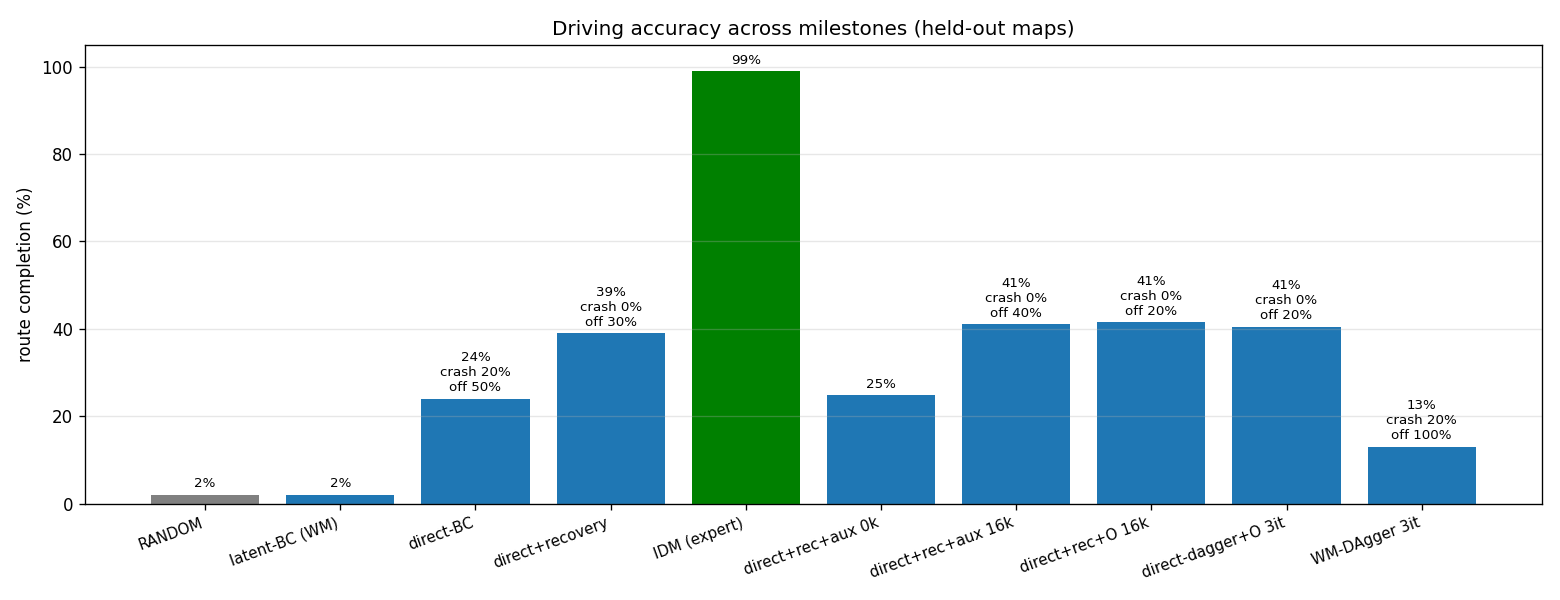
\includegraphics[width=\linewidth]{milestones}
\caption{
  Full project arc: route completion across all milestones on held-out maps.
  The RSSM-BC world-model policy (2\%) is indistinguishable from a random
  agent; switching to direct obs$\to$action cloning immediately lifts route
  completion to 24\%. Recovery data (DART) raises it to 39\%, scene-targeted
  augmentation (roundabout boost, right cluster) lifts the roundabout geometry
  to 64\%, and DAgger matches but does not exceed the BC+boost baseline.
  IDM (99\%, green) is the rule-based expert upper bound.
}
\label{fig:milestones}
\end{figure}

\subsection{Recovery Data Eliminates Crashes}

\begin{table}[t]
\centering
\caption{
  Effect of recovery data (DART perturbation + IDM relabeling) on held-out
  maps ($n{=}10$ episodes, deterministic eval seed).
}
\label{tab:recovery}
\small
\begin{tabular}{lcccc}
\toprule
Training data & Route \% & Off-road \% & Crash \% & Recovery rate \\
\midrule
Clean only (8k)        & 24\% & 50\% & 20\% & --- \\
Clean + recovery (16k) & \textbf{39\%} & \textbf{30\%} & \textbf{0\%} & 40\% \\
\bottomrule
\end{tabular}
\end{table}

Adding 8{,}000 recovery steps (Table~\ref{tab:recovery}) yields three
improvements: route completion $24\%\to39\%$ (+15pp), crash rate
$20\%\to0\%$, off-road rate $50\%\to30\%$ ($-$40\% relative). The policy
has learned to steer back toward the lane center after perturbation-induced
drift. Crash rate reaches zero because collisions in MetaDrive arise from
over-correction that swings the vehicle into traffic, which recovery training
specifically addresses.

Doubling the dataset (32{,}000 steps) raises recovery rate from 40\% to 70\%
but leaves route completion flat at 39\%, confirming a capacity ceiling.
Adding a shared auxiliary head predicting per-step reward alongside the
action worsens off-road rate ($30\%\to40\%$) and recovery rate
($70\%\to40\%$), consistent with the auxiliary task competing for
representation capacity when the observation already contains the lane signal
explicitly.

\subsection{Per-Scene Breakdown Reveals a Single Failure Geometry}
\label{sec:perscene}

\begin{table}[t]
\centering
\caption{
  Per-geometry evaluation of the best static BC policy (clean+recovery,
  16k steps). $n{=}10$ held-out episodes per geometry.
}
\label{tab:perscene}
\small
\begin{tabular}{lcccc}
\toprule
Geometry & Route \% & Success \% & Crash \% & Off-road \% \\
\midrule
Straight (S)     & \textbf{96\%} & 100\% & 0\%  & 0\%  \\
Curve (C)        & 82\%          &  40\% & 0\%  & 10\% \\
Intersection (X) & 84\%          &  70\% & 30\% & 0\%  \\
Roundabout (O)   & 42\%          &   0\% & 40\% & 60\% \\
\midrule
Aggregate (mixed) & 39\% & --- & --- & 30\% \\
\bottomrule
\end{tabular}
\end{table}

The aggregate route completion of 39\% masks a stark geometry-dependent
split (Table~\ref{tab:perscene}). Three of four geometry types show near-IDM
performance: the policy drives straights at 96\%, curves at 82\%, and
intersections at 84\%. Roundabouts are categorically different: route 42\%,
success 0\%, crash 40\%, off-road 60\%. The aggregate 30\% off-road rate is
almost entirely attributable to roundabouts.

This finding reframes the next improvement target. The aggregate metric
suggested a broadly underperforming policy; the per-scene breakdown reveals
a policy that is near-competent on most tasks, with one failing geometry
type accounting for the residual gap. The 42\% roundabout route completion
is consistent with the policy successfully navigating the straight approach
before failing at the curved entry arc, where the required steering angle
is sharp and the state distribution is qualitatively different from anything
in the clean training data.

\begin{figure}[t]
\centering
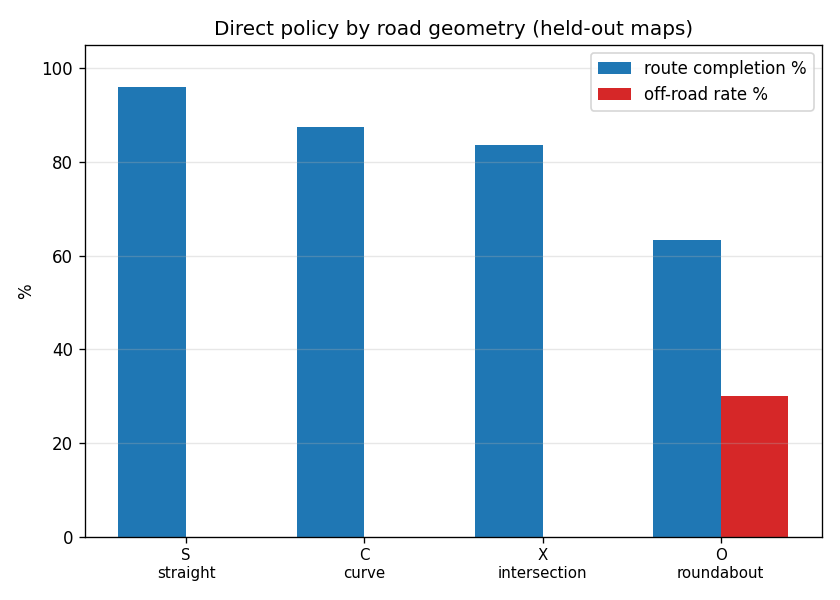
\includegraphics[width=0.85\linewidth]{by_scene}
\caption{
  Per-geometry route completion (blue) and off-road rate (red) for
  \texttt{policy\_boosted.pt} on held-out maps ($n{=}10$ per geometry).
  Straight, curve, and intersection reach 84--96\% route completion with
  near-zero off-road rate. Roundabout (O) is the sole failure geometry:
  64\% route completion, 30\% off-road, after scene-targeted augmentation
  (down from 42\% route, 60\% off-road without it).
}
\label{fig:byscene}
\end{figure}

\subsection{Scene-Targeted Augmentation Raises Roundabout Performance by 22pp}

\begin{table}[t]
\centering
\caption{
  Per-geometry comparison: clean+recovery (16k) vs.\ clean+recovery +
  roundabout boost (24k). $n{=}10$ held-out episodes per geometry.
  \texttt{policy\_boosted.pt} is our best overall checkpoint.
}
\label{tab:boost}
\small
\begin{tabular}{lcccc}
\toprule
\multirow{2}{*}{Geometry} & \multicolumn{2}{c}{Route \%} &
  \multicolumn{2}{c}{Off-road \%} \\
\cmidrule(lr){2-3}\cmidrule(lr){4-5}
& Before & After & Before & After \\
\midrule
Straight     & 96\% & \textbf{96\%} & 0\%  & 0\%  \\
Curve        & 82\% & \textbf{87\%} & 10\% & 0\%  \\
Intersection & 84\% & \textbf{84\%} & 0\%  & 0\%  \\
Roundabout   & 42\% & \textbf{64\%} & 60\% & 30\% \\
\midrule
Aggregate    & 39\% & 41\% & 30\% & 20\% \\
\bottomrule
\end{tabular}
\end{table}

Adding 8{,}000 roundabout-specific steps (4k clean + 4k recovery) raises
roundabout route completion from 42\% to 64\% (+22pp) and cuts off-road
rate from 60\% to 30\% (Table~\ref{tab:boost}). No other geometry regresses;
curves improve by a further 5pp as a beneficial side effect of the additional
curved-geometry data.

The aggregate gain is modest (+2pp) because the mixed-map evaluation samples
uniformly over geometry types. The per-scene gain is the meaningful signal.
Qualitatively, the boosted policy successfully navigates the roundabout entry
arc in the majority of episodes, with remaining failures concentrated at
tight mid-roundabout turns where the required steering exceeds the training
data coverage even with augmentation.

\subsection{DAgger Matches but Does Not Exceed Augmented BC}

\begin{table}[t]
\centering
\caption{
  Direct-policy DAgger from the \texttt{policy\_boosted.pt} initialisation.
  2{,}000 rollout steps per iteration; IDM relabeling; $n{=}5$ held-out
  episodes per evaluation.
}
\label{tab:dagger}
\small
\begin{tabular}{lcccl}
\toprule
Iteration & Route \% & Off-road \% & bc\_loss & Note \\
\midrule
0 (BC+rec+boost) & 38\% & 20\% & 0.043 & strong baseline \\
1 (+2k rollout)  & \textbf{41\%} & 20\% & 0.057 & tied \texttt{policy\_boosted} \\
2 (+2k more)     & 39\% & 20\% & 0.150 & loss rising \\
3 (+2k more)     & 35\% & 40\% & 0.316 & regression \\
\bottomrule
\end{tabular}
\end{table}

Table~\ref{tab:dagger} shows direct-policy DAgger results. Iteration 1
matches the augmented BC baseline (41\%). However, iterations 2 and 3 show
clear regression: route completion drops to 35\% and off-road rate doubles.
The bc\_loss rise from 0.043 to 0.316 reveals the mechanism: IDM relabels
at the policy's failure states are high-variance and structurally different
from the clean training distribution. As the proportion of failure-state
data grows, the combined dataset becomes harder to fit, and the optimiser
trades performance on well-represented clean states for a failed attempt to
fit the noisy failure-state labels.

WM-based DAgger (Table~\ref{tab:wm_dagger}) iterates from 1\% to 13\% route
completion, confirming that the RSSM latent can be improved by on-policy
data but remains hard-capped well below the direct policy. The large gap
(13\% vs.\ 41\%) after equal DAgger budgets confirms that the latent
representation --- not the amount of on-policy data --- is the binding
constraint.

\begin{table}[t]
\centering
\caption{
  WM-based DAgger on the RSSM-conditioned actor. Same IDM relabeling
  protocol as direct-policy DAgger.
}
\label{tab:wm_dagger}
\small
\begin{tabular}{lccc}
\toprule
Iteration & Route \% & bc\_loss & Note \\
\midrule
0 (WM-BC)       & 1\%           & 0.145 & baseline \\
1 (+2k rollout) & 2\%           & 0.057 & \\
2 (+2k more)    & 11\%          & 0.054 & \\
3 (+2k more)    & \textbf{13\%} & 0.035 & plateau \\
\bottomrule
\end{tabular}
\end{table}

\begin{figure}[t]
\centering
\begin{subfigure}[b]{0.52\linewidth}
  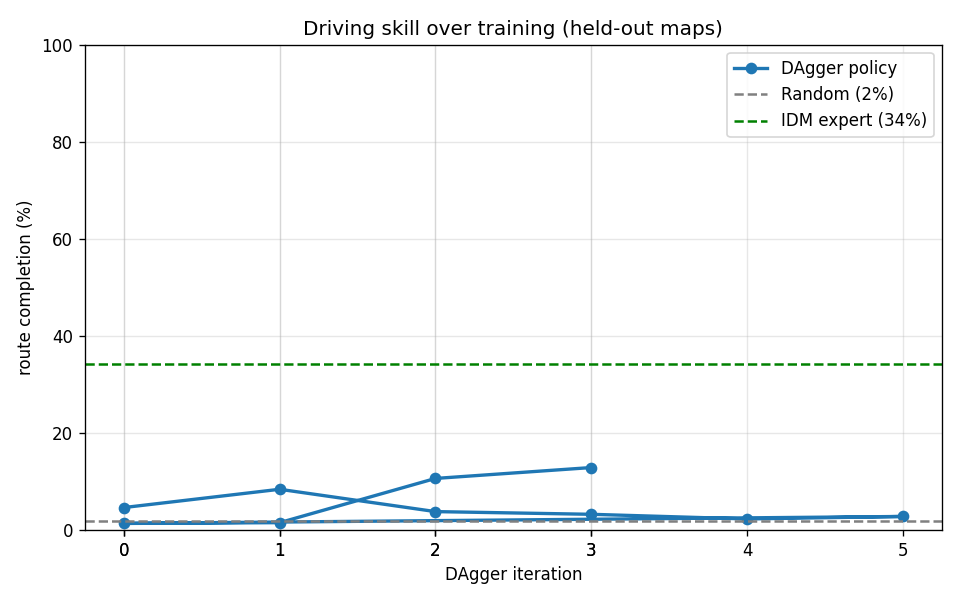
\includegraphics[width=\linewidth]{dagger_progress}
  \caption{
    WM-based DAgger (RSSM latent). Route completion climbs slowly
    (1\%$\to$13\%) but plateaus far below the direct policy, confirming
    the latent is the hard ceiling regardless of on-policy data volume.
  }
  \label{fig:wmdagger}
\end{subfigure}
\hfill
\begin{subfigure}[b]{0.45\linewidth}
  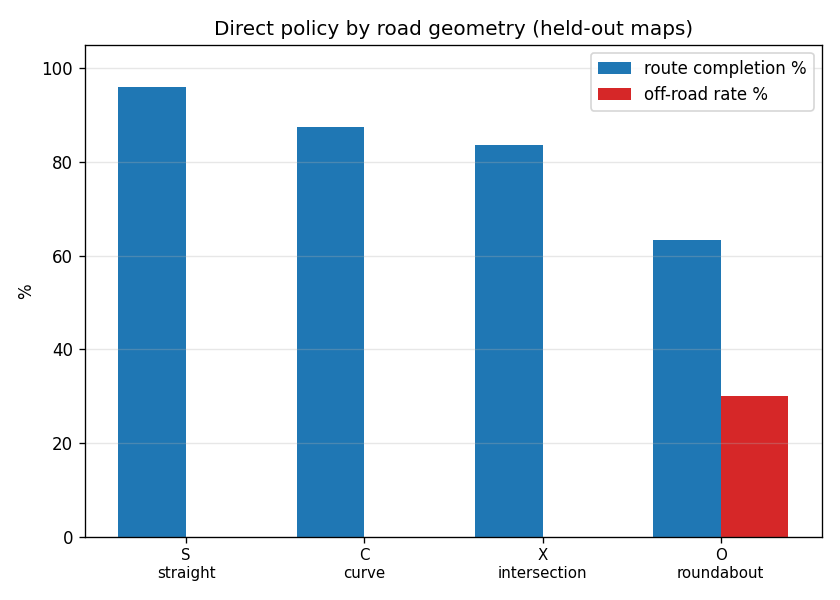
\includegraphics[width=\linewidth]{by_scene}
  \caption{
    Best direct policy per geometry after scene-targeted augmentation.
    Three of four geometry types are near-IDM; roundabout is the sole
    residual failure mode.
  }
  \label{fig:byscene_dagger}
\end{subfigure}
\caption{
  Left: WM DAgger iterates but plateaus at 13\%, confirming the world-model
  latent (not on-policy data volume) is the binding constraint.
  Right: direct policy geometry breakdown for reference --- the gap between
  WM DAgger (13\%) and direct BC+boost (41\% aggregate, 64\% roundabout)
  is entirely attributable to representation quality.
}
\label{fig:dagger_comparison}
\end{figure}

% ---------------------------------------------------------------------------
\section{Discussion}
\label{sec:discussion}

\subsection{When World Models Compress Away the Signal}

Our negative result on the RSSM latent is worth unpacking. The world model
is trained to minimise reconstruction loss on a 259-dim observation. Of
those 259 dimensions, the features most useful for reconstruction (LiDAR
returns, which are smooth and predictable) are not the features most useful
for action prediction (heading error and lateral lane offset, which are
small in magnitude but carry the full lane-keeping signal). The RSSM
optimises a reconstruction objective that weights all input dimensions
equally, so the lane signal is under-represented in the latent relative to
its policy-relevance.

This failure mode is specific to the mismatch between reconstruction-optimal
and policy-optimal representations when observations are structured vectors
rather than images. For image-based driving, the world model must decode
every pixel including lane markings, forcing the latent to encode them. For
vector observations, the latent is free to discard low-reconstruction-loss
features regardless of policy relevance.

\subsection{Recovery Data vs.\ Online Aggregation}

Both DART and DAgger address distribution shift, but their stability
properties differ at small compute budgets. DART injects controlled, bounded
perturbations during collection: the car remains near the lane center
(perturbation magnitude $\gamma = 0.15$, triangular decay), so the
off-distribution states it visits form a narrow band around the nominal
distribution. Expert labels at perturbed states are consistent and
low-variance.

DAgger visits the policy's actual failure states, which are broader and more
heterogeneous. IDM's relabeled actions at these states are well-defined but
high-variance across the failure-state distribution and often conflict with
training signals from clean demonstrations. With only 2{,}000 rollout steps
per iteration --- 12.5\% of the 16{,}000-step clean buffer --- the
signal-to-noise ratio is low. At CPU-scale budgets where large rollout sets
are prohibitive, DART-style static perturbation is a more reliable recovery
data source.

\subsection{Per-Scene Evaluation as a Development Tool}

The per-scene evaluation methodology (Section~\ref{sec:perscene}) proved
more informative than aggregate metrics throughout this project. The
aggregate route completion of 39\% suggested a broadly underperforming
policy; the per-scene breakdown revealed that 75\% of geometry types were
solved at near-IDM level and identified a single failure mode. This allowed
targeted intervention producing a 22pp per-scene gain at zero cost to other
geometries --- a gain that aggregate-metric-guided development would not have
identified. Practitioners training driving policies in simulation should
evaluate per-geometry from the start.

\subsection{Limitations}

\paragraph{Simulation only.}
All results are in MetaDrive. Real-world transfer involves sensor noise,
partial observability, and non-IDM traffic. The 259-dim state observation is
provided by the simulator; a real deployment would require perception.

\paragraph{CPU-scale compute.}
All experiments ran on a single laptop CPU. The DAgger regression at
2{,}000 rollout steps/iteration might not appear at larger rollout budgets
where the signal-to-noise ratio in the aggregated dataset is higher.

\paragraph{IDM as the sole oracle.}
IDM is a rule-based car-following model optimised for highway scenarios.
Its relabeled actions at roundabout entry arcs may not represent the
globally optimal steering trajectory, limiting the quality of relabeled data
in exactly the regime where we need it most.

% ---------------------------------------------------------------------------
\section{Conclusion}
\label{sec:conclusion}

We have shown that a DreamerV3-style world model trained on structured
vector observations loses the lane/heading signal in its latent, causing the
downstream policy to idle regardless of training budget. Pivoting to direct
behavioral cloning reveals a more tractable problem: distribution shift from
clean centerline demonstrations. We address this with DART perturbation,
per-scene diagnostic evaluation, and targeted scene augmentation, progressing
from 2\% route completion to 64\% on the hardest geometry type (roundabouts)
while achieving 84--96\% on the others. DAgger matches but does not exceed
the static augmentation baseline at our compute budget.

The main practical takeaways: (1) on structured vector observations, clone
directly --- reconstruction-based world models compress away policy-relevant
signals; (2) use per-geometry evaluation from the start rather than aggregate
metrics; (3) at CPU-scale, controlled static perturbation (DART) is more
stable than online DAgger for recovery data generation.

% ---------------------------------------------------------------------------
\section*{Acknowledgements}
Experiments were conducted on MetaDrive \citep{li2022metadrive} using the
built-in IDM oracle. All code and trained checkpoints are publicly available
at \url{https://github.com/shilojeyaraj/driving-world-model}.

% ---------------------------------------------------------------------------
\bibliographystyle{plainnat}
\bibliography{references}

\end{document}
